\documentclass[a4paper,12pt]{article}

\usepackage{natbib,setspace,amsmath,graphicx,float,booktabs}
\usepackage[skip=0.5\baselineskip]{caption}
\usepackage[title]{appendix}
\bibliographystyle{unsrtnat}

\onehalfspacing
\newcommand{\bs}[1]{\boldsymbol{#1}}
\setlength\parindent{0pt}

\begin{document}

\begin{titlepage}
\noindent
\includegraphics[width=5cm]{uzh_logo_e_pos.pdf}
\noindent{\bf Department of Economics}
\noindent\rule{\textwidth}{0.4pt}
\vspace{1cm}
  \begin{center}
		{\LARGE Using AS-AD framework and VAR model to [...] Interwar US} \\
		{\Large Quantitative Economic History - Applications\\Spring Term 2021}
  \end{center}
\vfill

{\flushleft
Hubert Mrugala \\
Banking and Finance\\
hubert.mrugala@uzh.ch\\
19764265}  

\end{titlepage}

\pagebreak
\pagebreak

\section{Introduction}

Aaa.
\newpage

\section{Data}

The dataset consists of 252 monthly observations of American Industrial Production (IP) and Consumer Index Prices (CPI) from January 1919 to December 1939. The data can be split into two periods, i.e. pre-Great Depression and Great Depression. The first one I define as the time between the beginning of the data sample, January 1919, to the upper-turning point in May 1929, the second one follows from that point to the end of the time-series. On figure \ref{fig:fig1} and figure \ref{fig:fig2} the two periods are separated by a red vertical line Some simple statistics are shown in the table below, and a table with yearly data for the time-series can be found in the appendix. 

\begin{table}[h]
\label{table:1}
\caption{Basic Statistics}
\centering
\input{../output/tables/stats.txt}
\end{table}

After the war there was a sharp increase in the price level index from 57 in the beginning of 1919 to 70 in mid 1920s. Then, prices had deflated to about 59 (Depression of 1920-21) and stayed around that level until the Great Depression. In February 1931 CPI dropped below 55. Not surprisingly years 1931-33 are considered to be the most severe time of the Great Depression as in this period prices were declining each month until reaching the lowest point of 43.7 in April 1933.

\begin{figure}[H]
    \centering
\caption{Consumer Price Index}
\label{fig:fig1}
    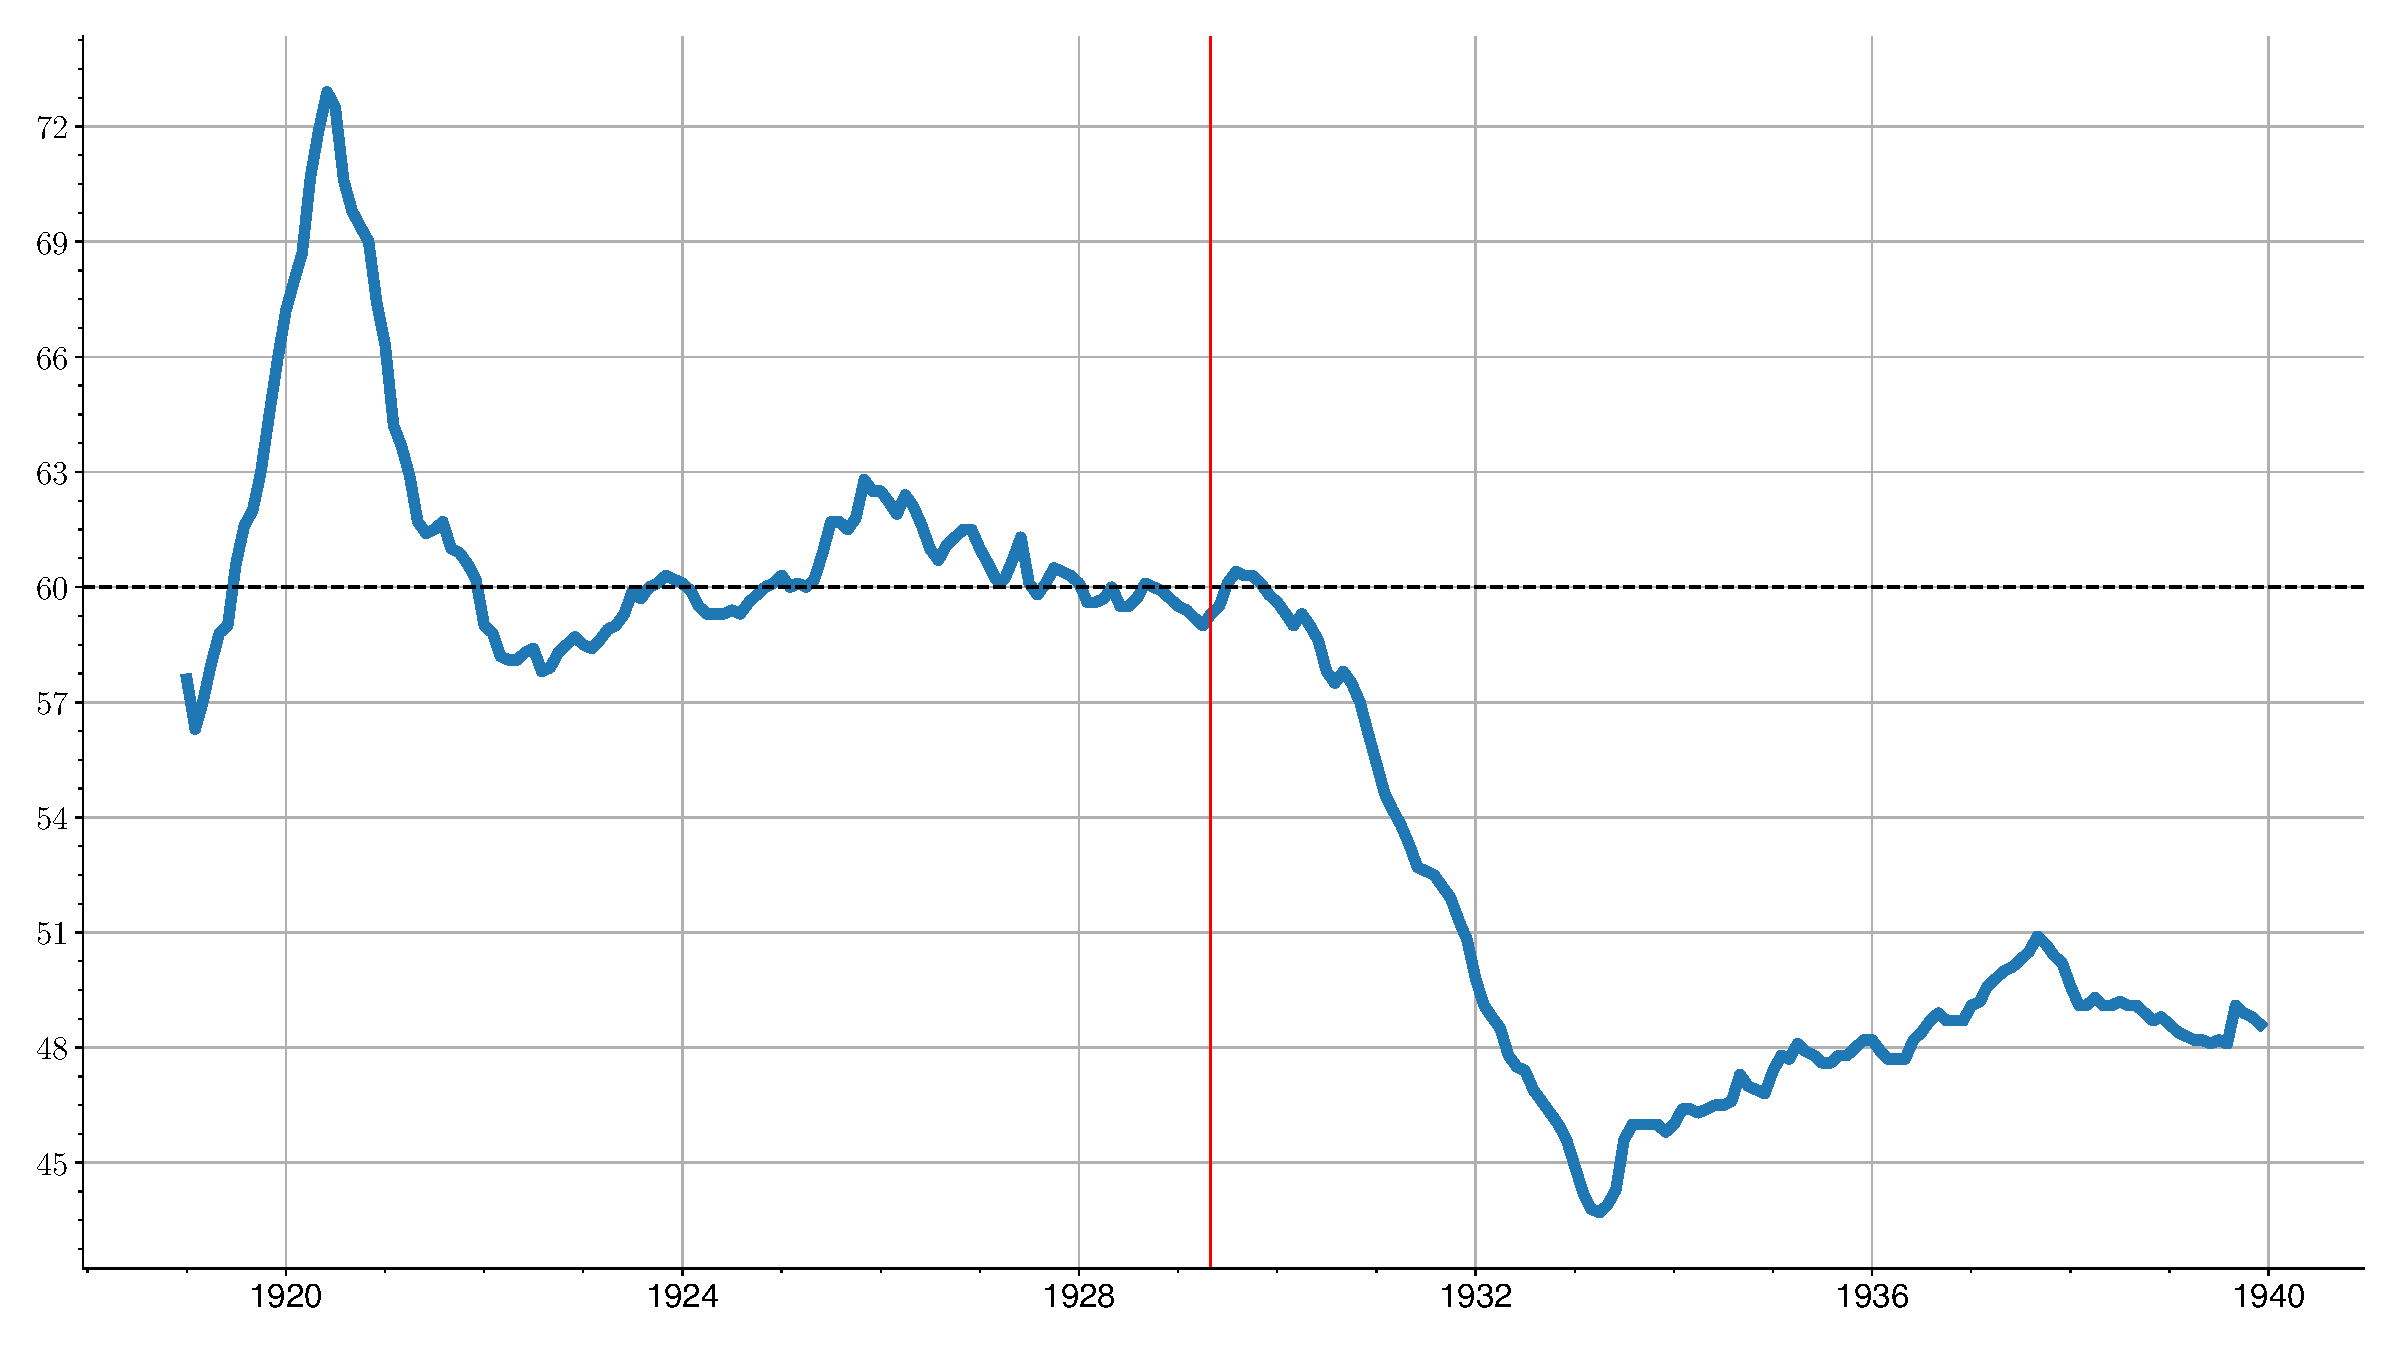
\includegraphics[width=\textwidth]{../output/figures/ts_CPI.pdf} 
\end{figure}

Pre-Great Depression Industrial Production, except the time of 1920-21 depression, was growing steadily. At the peak, IP was about 40 and it took almost 7 years of depression and recovery to come back to that level. Recovered production didn't stay that high for long. At the end of the inter-war period we can see a very sudden collapse of IP. It is the Recession of 1937-38, according to \cite{bordo2012}, the third-worst contraction of the twentieth century. 

To better understand the business cycle in the interwar United States I detrended the time-series with a Hodrick-Prescot filter (see Figure \ref{fig:fig2}. For the smoothing parameter I went with recommendation of \cite{morten1997} and set \(\mu\) to 129600. There were five periods when Industrial Production deviated by more than 5 points from the trend. However, the most distinct seems to be the interval from 1930 to 1933 when not only the cycle component but also the trend component was falling for a prolonged period of time. 

\pagebreak

\begin{figure}[t]
    \centering
\caption{Industrial Production}
\label{fig:fig2}
    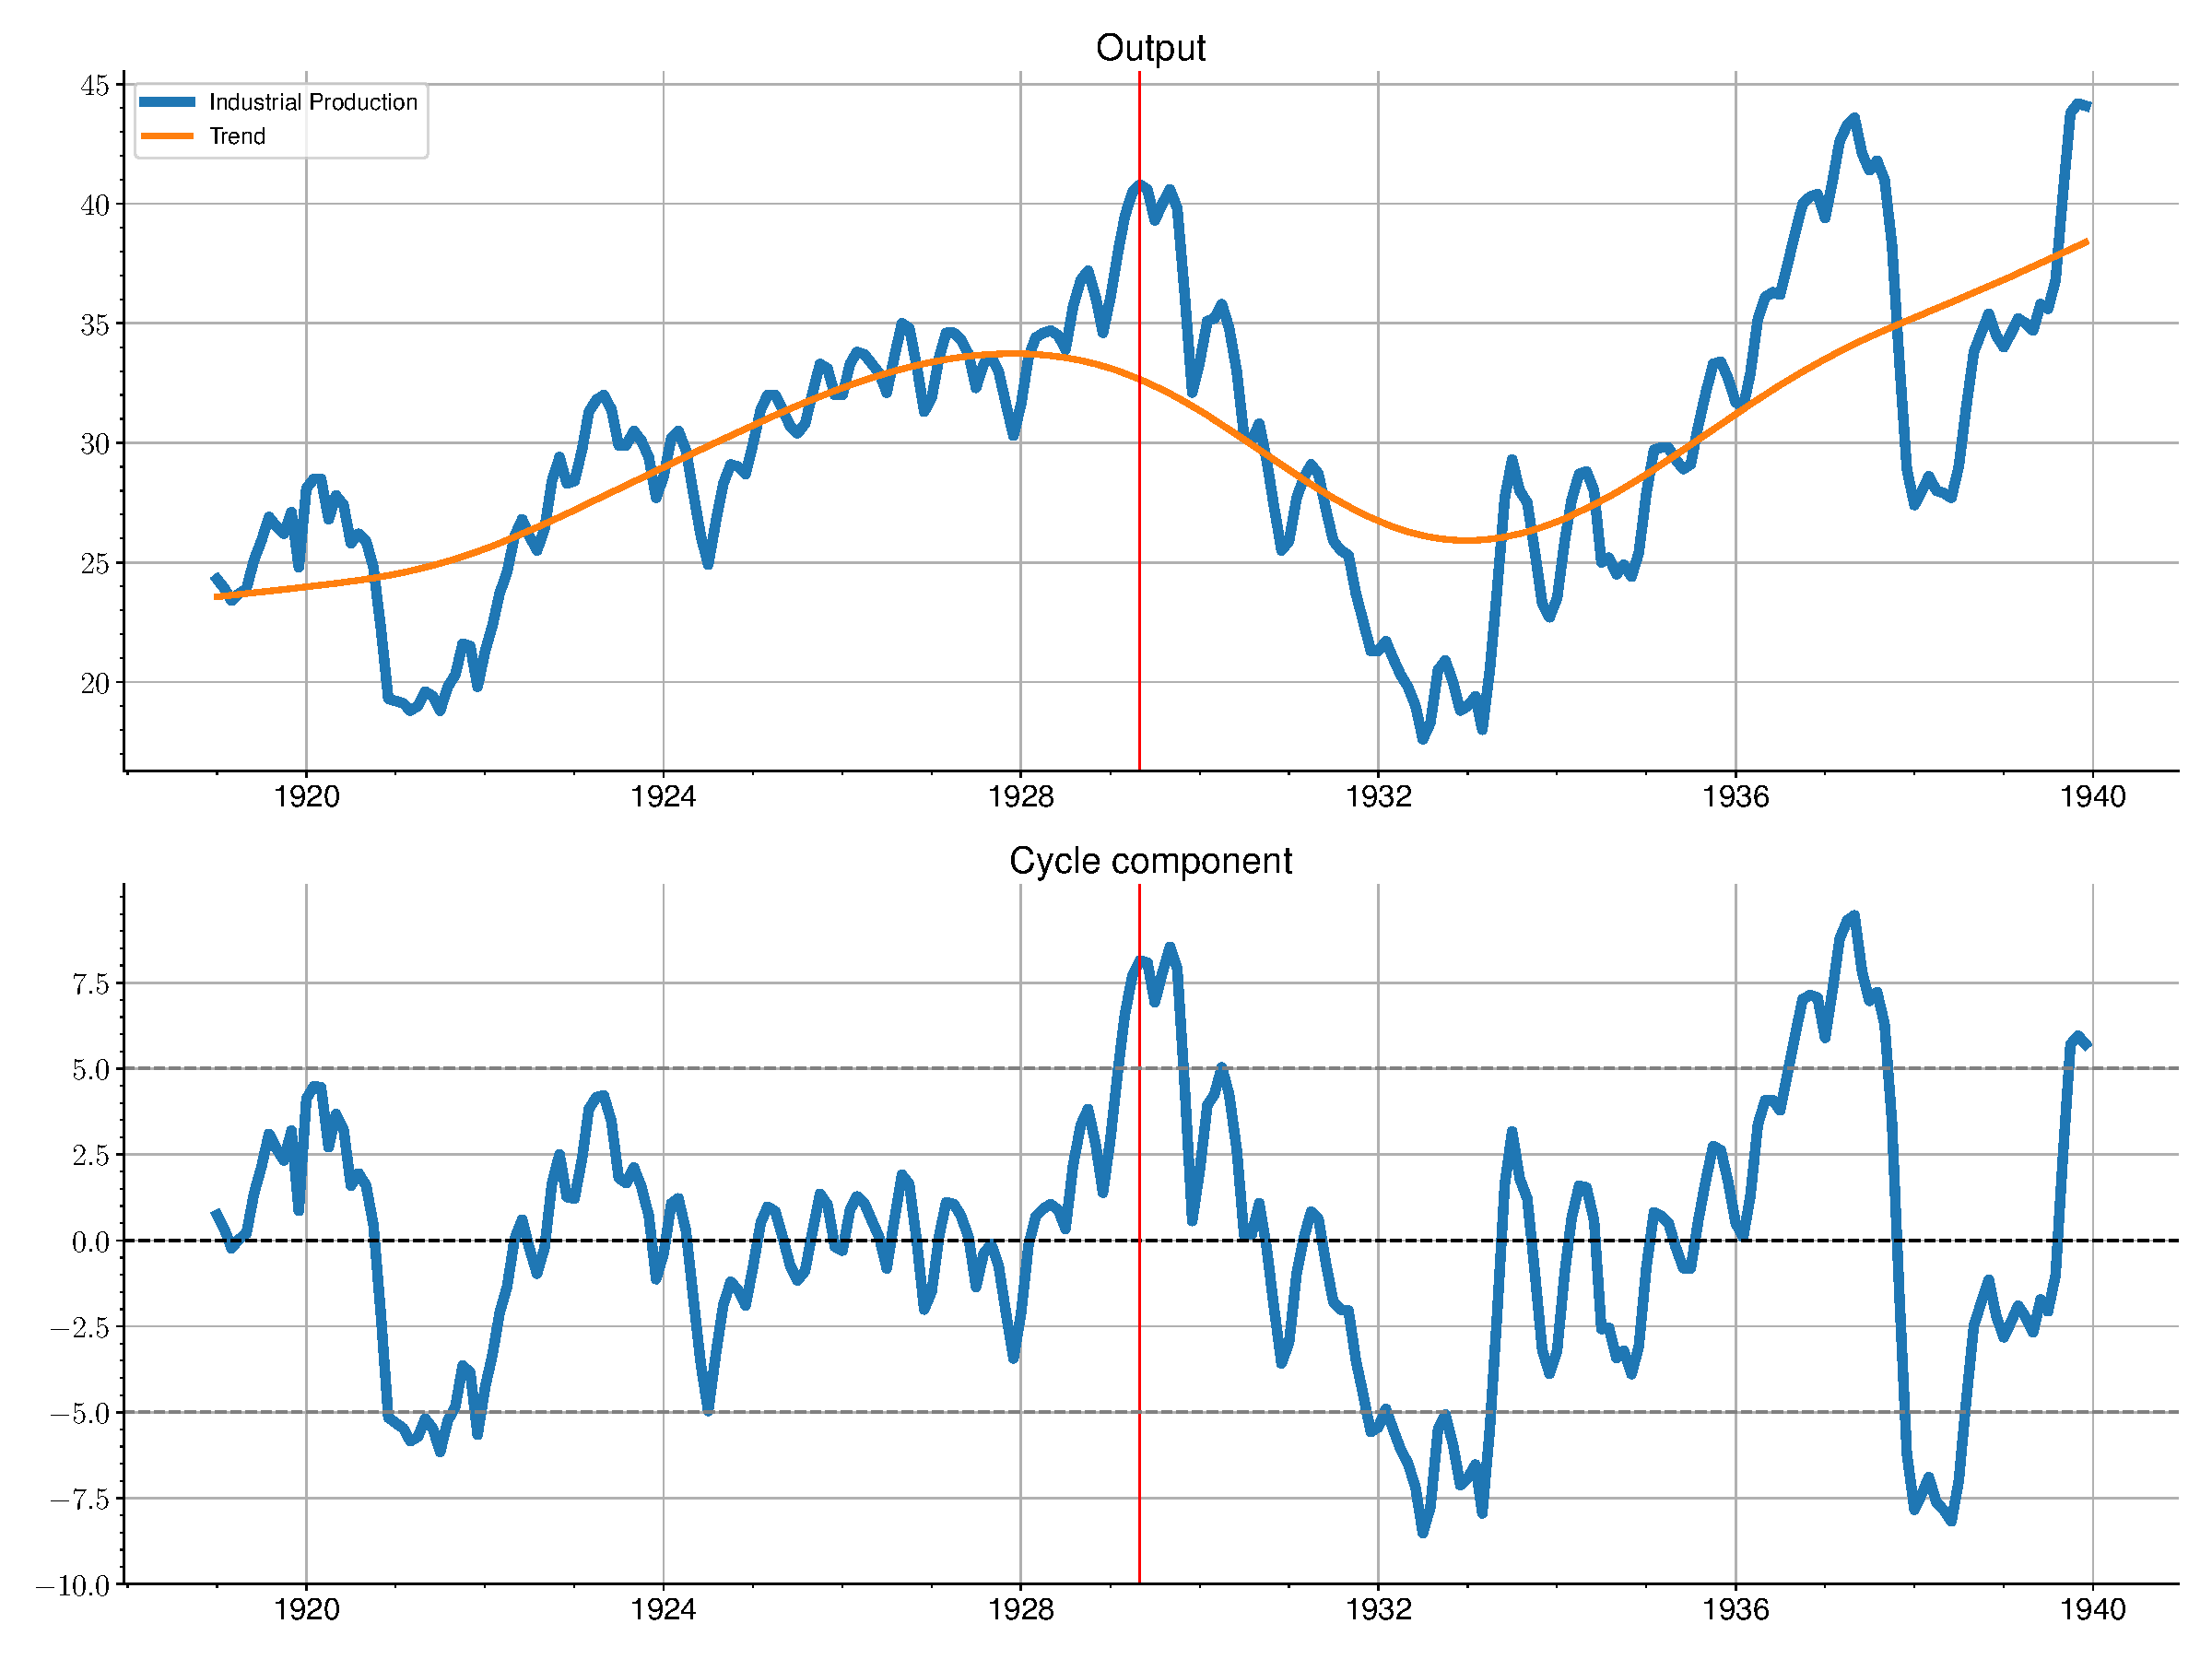
\includegraphics[width=\textwidth]{../output/figures/ts_IP.pdf} 
\end{figure}

The dataset comes from:
\begin{itemize}
		\item Statistisches Handbuch der Weltwirtschaft (1936), bearb. im statistischen Reichsamt
Verlag für Sozialpolitik, Wirtschaft und Statistik GmbH, Berlin.
\end{itemize}
 

\section{Method}
\subsection{Vector Autoregressive Model}

To analyze relationship between two endogenous time-series, price level \(\bf M\) and output \(\bf Y\), a vector autoregression (VAR) model is used.

\begin{equation} \label{eq:1}
		{\mathbf{y_{t}=c+A_{1}y_{{t-1}}+A_{2}y_{{t-2}}+\cdots +A_{p}y_{{t-p}}+e_{t}}}
\end{equation}

In the formula above \(\bf c\) is a constant, \(\bf A_i\) are coefficient matrices and \(\bf u_i\) are error terms. When analyzing monetary transmission mechanism, VAR can be also expressed in the following form \citep{favero2001}

\begin{equation} \label{eq:2}
\begin{split}
		\mathbf{G}\left(\begin{array}{c}
		\mathbf{Y}_{t} \\
		\mathbf{M}_{t}
		\end{array}\right)=\mathbf{K}(L)\left(\begin{array}{c}
		\mathbf{Y}_{t-1} \\
		\mathbf{M}_{t-1}
		\end{array}\right)+\mathbf{F}\left(\begin{array}{c}
		\epsilon_{\mathbf{Y}, \mathbf{t}} \\
		\epsilon_{\mathbf{M}, \mathrm{t}}
		\end{array}\right).
\end{split}
\end{equation}

In the structural model above matrix \(\bf G\) represents contemporaneous relations among the variables and \(\bf K(L)\) is the matrix of finite-order lag polynomial. The model is not directly observable, however, a reduced form can be estimated.

\begin{equation} \label{eq:3}
\begin{split}
		\left(\begin{array}{c}
		\mathbf{Y}_{t} \\
		\mathbf{M}_{t}
		\end{array}\right)=\mathbf{G}^{-1} \mathbf{K}(L)\left(\begin{array}{c}
		\mathbf{Y}_{t-1} \\
		\mathbf{M}_{t-1}
		\end{array}\right)+\mathbf{G}^{-1} \mathbf{F}\left(\begin{array}{c}
		\epsilon_{\mathbf{Y}, \mathbf{t}} \\
		\epsilon_{\mathbf{M}, \mathrm{t}}
		\end{array}\right)
\end{split}
\end{equation}

In this paper, vector autoregression is used to obtain impulse responses and forecast error decomposition in the AS-AD framework. To do this, I use Blanchard-Quach decomposition where we assume that aggregate demand shocks has no long-run effect on real output \citep{blanchardquah89}. The assumption helps to solve the identification problem by imposing restictions on the impact matrix \(\bf S = G^{-1}-F\)

\begin{equation} \label{eq:4}
		\mathbf{u}_{\mathbf{t}}=\mathbf{S} \epsilon_{\mathbf{t}}
\end{equation}

To find \(\bf S\), first lets start with the moving average representations of reduced form VAR (equation 1) and the structural model (equation 2).

\begin{equation} \label{eq:5}
\begin{split}
		\mathbf{y}_{\mathbf{t}} &=\mathbf{B}(\mathbf{L}) \mathbf{u}_{\mathbf{t}}, \\
		\mathbf{y}_{\mathbf{t}} &=\mathbf{C}(\mathbf{L}) \epsilon_{\mathbf{t}}
\end{split}
\end{equation}

After substituting for \(\bf u_t\) and simplifying

\begin{equation} \label{eq:6}
		\mathbf{B}(L) \mathbf{S}=\mathbf{C}(L)
\end{equation}

The long-run coefficient matrix is \(\bf C(1) = B(1)S\), and so to get \(\bf S\), long-run \(\bf C(1)\) is needed. Postmultiplying \(\bf C(1)\) with its transpose gives

\begin{equation} \label{eq:7}
		\mathbf{B}(1) \mathbf{S S}^{\prime} \mathbf{B}(1)^{\prime}=\mathbf{C}(1) \mathbf{S}^{-1} \mathbf{S} \mathbf{S}^{\prime}\left(\mathbf{S}^{\prime}\right)^{-1} \mathbf{C}(1)^{\prime}=\mathbf{C}(1) \mathbf{C}(1)^{\prime}.
\end{equation}

Cholesky decomposition of the expression above produces the restricted long-run coefficient matrix \(\bf C(1)\), that allows to calculate matrix \(\bf S\).

\subsection{Impulse Responses}

Impact matix \(\bf S\) connects structural shocks \(\bf e_t\) to the reduced form residuals \(\bf u_t\)

\begin{equation} \label{eq:8}
		\mathbf{u}_{\mathbf{t}}=\mathbf{S} \epsilon_{\mathbf{t}}
\end{equation}

To find S first lets start with the moving average representations of reduced form VAR equation 1 and the structural model eq2.

\begin{equation} \label{eq:9}
\begin{split}
		\mathbf{y}_{\mathbf{t}} &=\mathbf{B}(\mathbf{L}) \mathbf{u}_{\mathbf{t}}, \\
		\mathbf{y}_{\mathbf{t}} &=\mathbf{C}(\mathbf{L}) \epsilon_{\mathbf{t}}
\end{split}
\end{equation}

After substituting for u t and simplifying

\begin{equation} \label{eq:10}
		\mathbf{B}(L) \mathbf{S}=\mathbf{C}(L)
\end{equation}

The long-run coefficient matrix is \(\bf C(1) = B(1)S\), and so to get \(\bf S\), long-run \(\bf C(1)\) is needed. Postmultiplying C(1) with its transpose gives

\begin{equation} \label{eq:11}
		\mathbf{B}(1) \mathbf{S S}^{\prime} \mathbf{B}(1)^{\prime}=\mathbf{C}(1) \mathbf{S}^{-1} \mathbf{S} \mathbf{S}^{\prime}\left(\mathbf{S}^{\prime}\right)^{-1} \mathbf{C}(1)^{\prime}=\mathbf{C}(1) \mathbf{C}(1)^{\prime}.
\end{equation}

Cholesky decomposition of the expression above produces the restricted long-run coefficient matrix \(\bf C(1)\), that allows to calculate matrix \(\bf S\).

\subsection{Forecast Error Variance Decomposition}

Forecast error variances for two variables \((k=1,2)\) can be expressed as

\begin{equation} \label{eq:12}
		\mathrm{E}\left[\left(y_{k, t+1}-\hat{y}_{k, t+1}\right)^{2}\right]=\mathbf{e}_{k} \mathbf{\Sigma} \mathbf{e}_{k}^{\prime}=\mathbf{e}_{k} \mathbf{S S}^{\prime} \mathbf{e}_{k}^{\prime}=\mathbf{e}_{k} \mathbf{C}_{0} \mathbf{C}_{0}^{\prime} \mathbf{e}_{k}^{\prime}.
\end{equation}

Then contribution of the the shock \(l\) to the forecast error variances of variable \(k\) at time \(h\) can be, generally, written in a for of the following three dimentional array

\begin{equation} \label{eq:13}
		\theta_{h, k l}=\frac{\sum_{j=0}^{h-1}\left(\mathbf{e}_{k} \mathbf{C}_{j} \mathbf{e}_{l}^{\prime}\right)^{2}}{\sum_{j=0}^{h-1} \mathbf{e}_{k} \mathbf{C}_{j} \mathbf{C}_{j}^{\prime} \mathbf{e}_{k}^{\prime}}
\end{equation}

\newpage

\section{Results}

\begin{table}
\label{table:3}
\caption{Restricted Long-run Responses}
\centering
\input{../output/tables/C1.txt}
\end{table}

\begin{itemize}
\item Price index:
\begin{itemize}
\item 1700-1823: \citet{schumpeter38}, in \citet[p. 468-469]{mitchelldeane71}
\item 1823-1913: \citet[p. 863-864]{mitchelle2003}
\end{itemize}

\item Industrial production: \citet[p. 725-727]{craftsharley92}

\end{itemize}

\begin{figure}[H]
    \centering
\caption{Impulse Responses}
    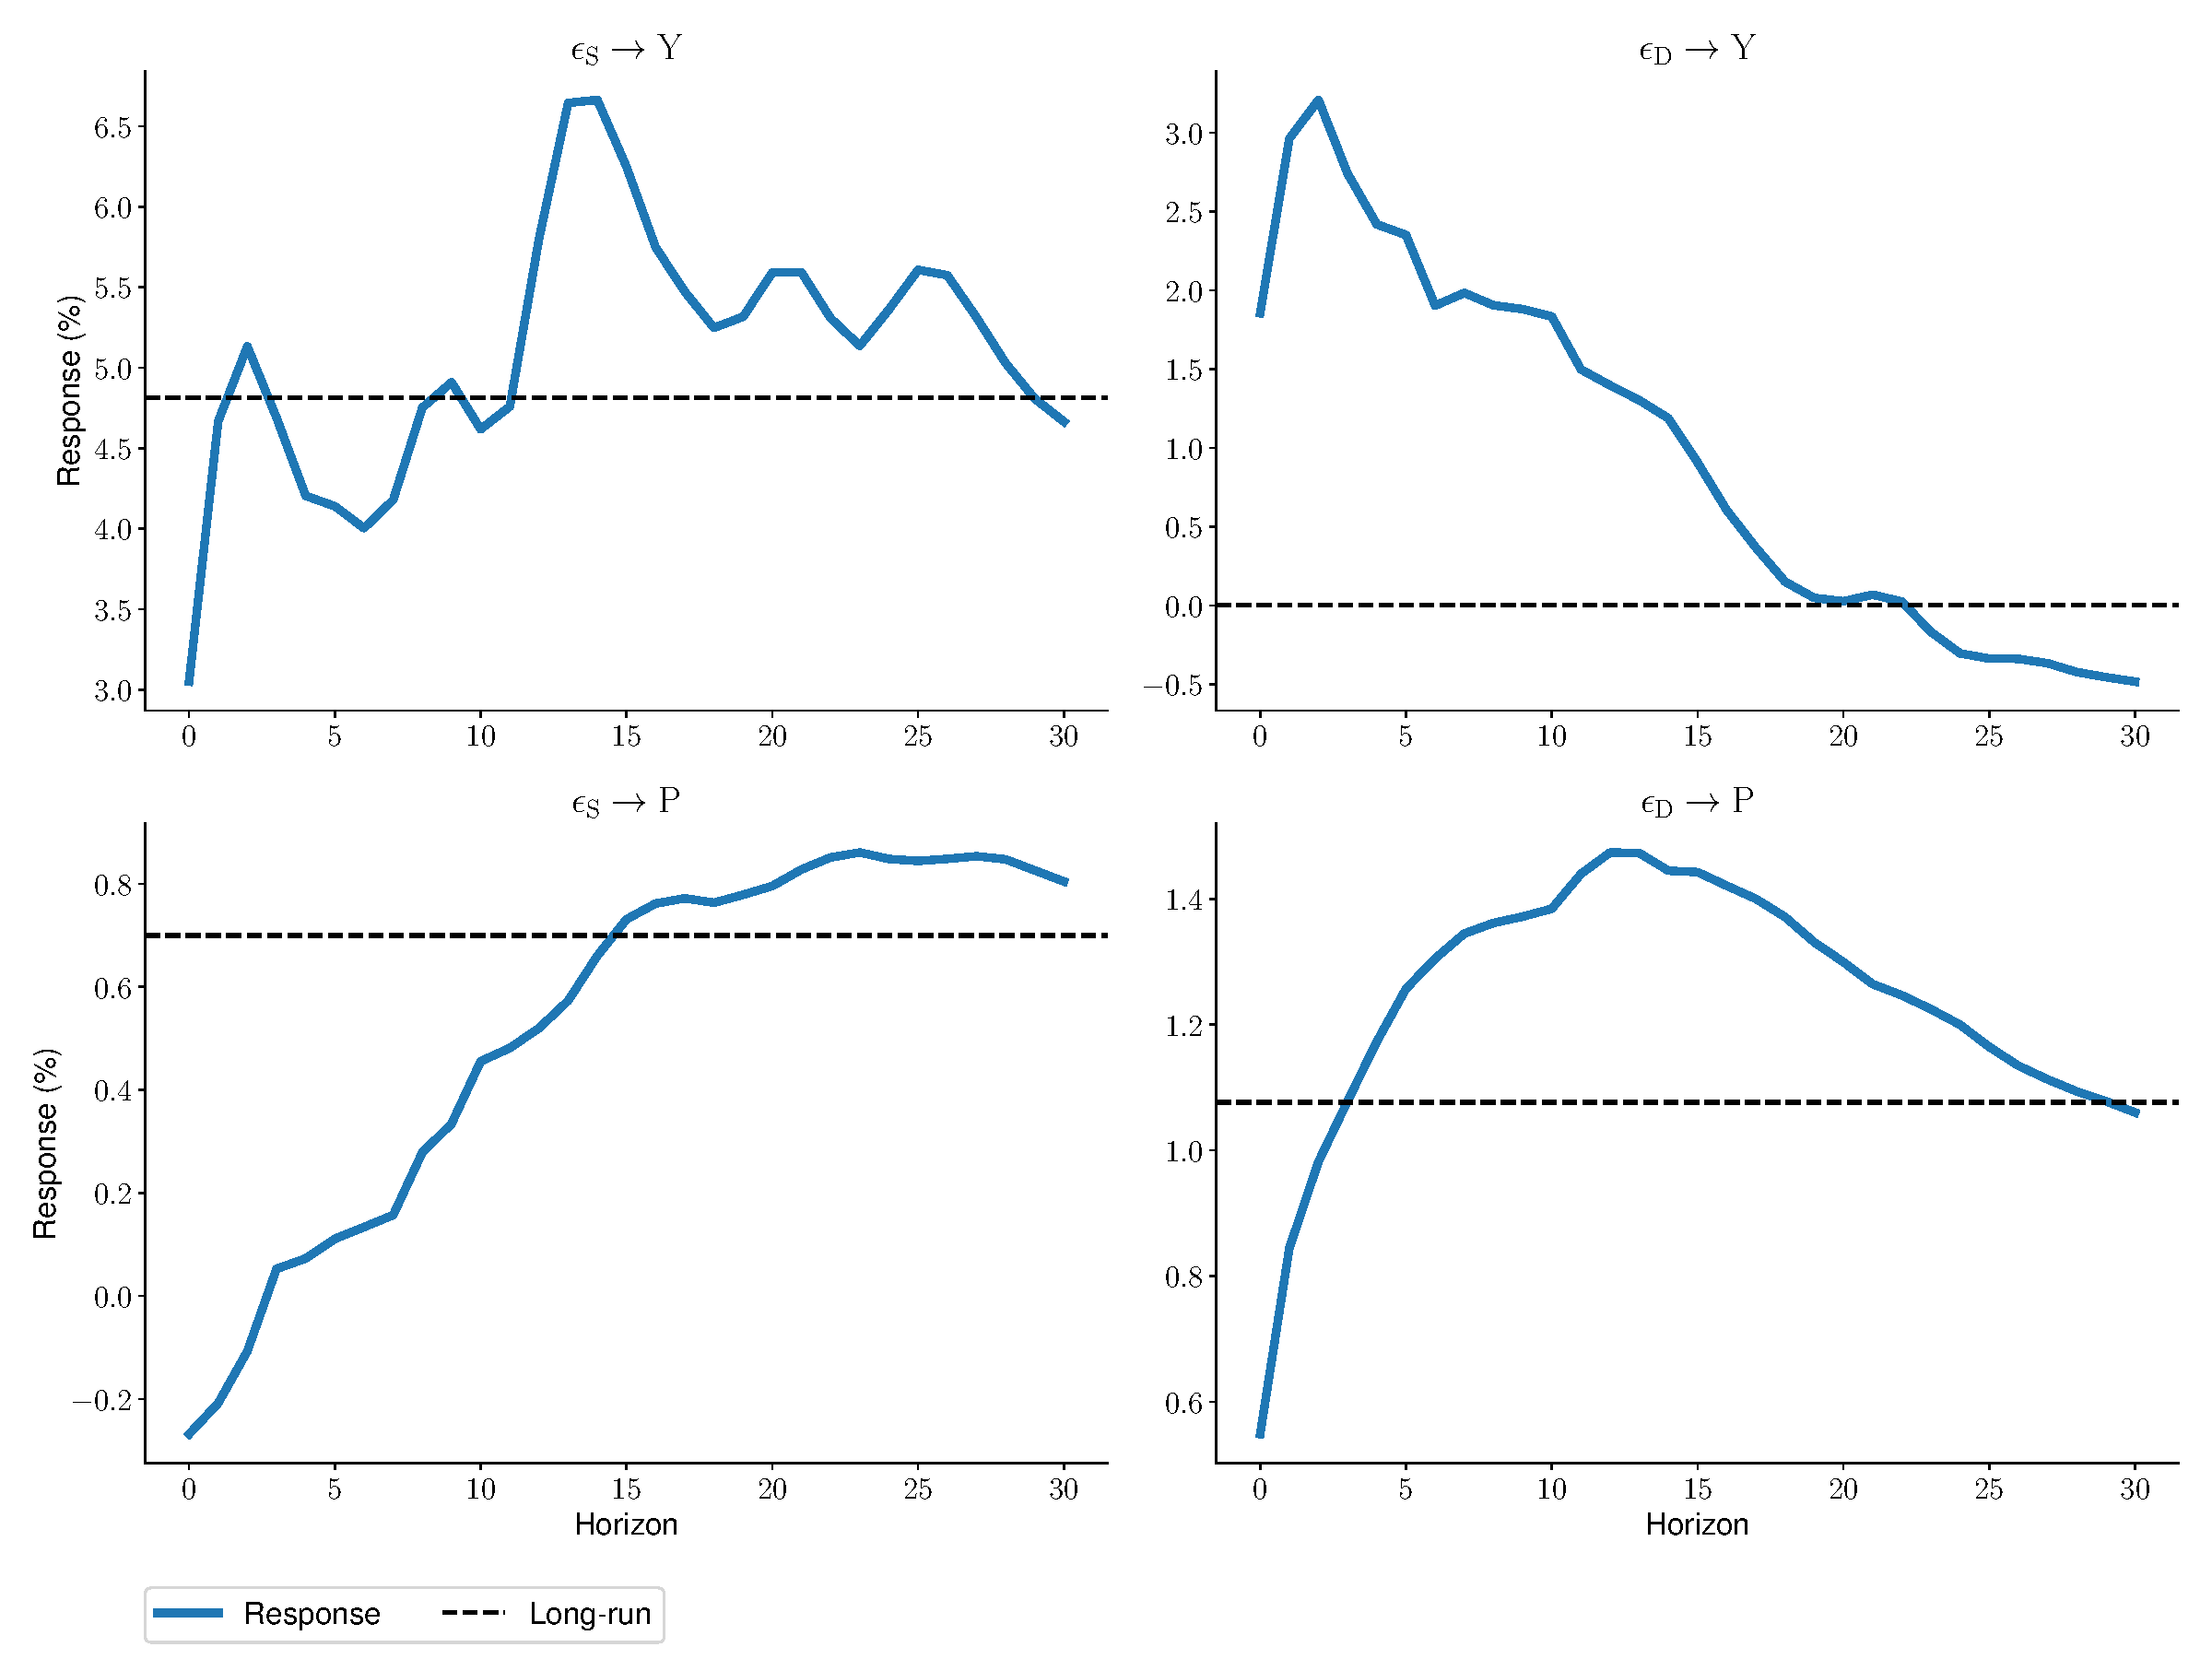
\includegraphics[width=\textwidth]{../output/figures/IR.pdf} 
\end{figure}

To be discussed.

\pagebreak

\begin{appendices}
\section{Yearly Data}

\begin{table}[h]
\centering
\input{../output/tables/yearly_data.txt}
\end{table}

\end{appendices}

\pagebreak

\bibliography{bib}

\end{document}
